\documentclass[12pt,spanish]{article}
\usepackage[utf8]{inputenc}
\usepackage[spanish]{babel}
\usepackage{graphicx}
\usepackage{amsmath}
\usepackage{moreverb}
\usepackage{float}

\begin{document}

\begin{center}
  \textbf{\Huge Universidad de Sonora}\\[0.5cm]
  {\LARGE División de Ciencias Exactas y Naturales}\\[0.5cm]
  {\LARGE Departamento de Física}\\[1.25cm]
    \includegraphics[width=3.5cm,height=3.5cm]{unison.jpeg}\\[0.8cm]
     \vfill
  {\Large Reporte de Actividad 3}\\[2.1cm]
  {\Large \textbf{\Huge Interpolación}}\\[3.0cm]
  {\Large Estefania Eng Duran}\\[2.1cm]
  Física Computacional I 2016-1\\[0.5cm]
  Hermosillo - \today
\end{center}

\section*{Introducción}

La interpolación es un método en el que se construyen nuevos datos a partir de un conjunto discreto de datos conocidos. En el campo de de la ciencia e ingeniería, con frecuencia se obtienen datos mediante experimentación o muestreo que representan los valores de una función y se requiere estimar el valor de la función para un valor intermedio de la variable independiente. Lo que se hace es se construye una curva o superficie que une los puntos donde se han realizado las mediciones y cuyo valor sí se conoce. Algunas formas de interpolación que se utilizan con frecuencia son la interpolación polinómica, la interpolación por medio de spline o la interpolación polinómica de Hermite.

En esta actividad aprenderemos acerca del proceso de encontrar una función que interpole los puntos, con ayuda de la función \textbf{scipy.interpolate} de Python. Hay varios servicios de interpolación disponibles en SciPy, en esta ocasión usaremos la clase \textbf{interp1d} la cual es un método conveniente para crear una función a partir de puntos fijos que puede ser evaluada en cualquier parte del dominio definido por los datos dados usando interpolación lineal. Lo que hace \textbf{interp1d} es interpolar una función 1-D. Esta función toma valores $x$ y $y$ los cuales son arreglos que son utilizados para aproximarse a alguna función f: y= f(x).


\bigskip

\section*{Actividad}

El siguiente ejemplo demuestra el uso de \textbf{interp1d} para interpolación lineal, aproximal, zero-padding y spline del primero, segundo, tercero y décimo orden.

\clearpage

\paragraph{Código Ejemplo}

\begin{center}
\begin{boxedverbatim}
import numpy as np
import matplotlib.pyplot as plt
from scipy.interpolate import interp1d

# Original "data set" --- 21 random numbers between 0 and 1.
x0 = np.linspace(-1,1,21)
y0 = np.random.random(21)

plt.plot(x0, y0, 'o', label='Data')

# Array with points in between those of the data set for
# interpolation.
x = np.linspace(-1,1,101)

# Available options for interp1d
options = ('linear', 'nearest', 'zero', 'slinear',
           'quadratic', 'cubic', 10)

for o in options:
    f = interp1d(x0, y0, kind=o)  # interpolation function
    plt.plot(x, f(x), label=o)    # plot of interpolated data

plt.legend()
plt.show()
\end{boxedverbatim}
\end{center}

\begin{figure}[H]
    \centering
	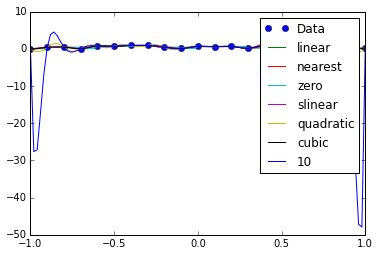
\includegraphics[height=7.5cm]{original.png}
    \caption{Resultado del código original}
\end{figure}

\bigskip

Los ejercicios de esta actividad nos pide realizar una interpolación lineal, cuadrática y cúbica de una serie de datos generados de manera aleatoria dentro de un rango y en base a una función. A continuación modificamos el código original para cada uno de los siguientes cuatro casos.

\newpage

\paragraph{Caso 1}

Dados 10 puntos aleatorios entre $x=0$ y $x=3$ para la función $f(x) = sin(2 x)$.

\begin{center}
\begin{boxedverbatim}

import numpy as np
import matplotlib.pyplot as plt
from scipy.interpolate import interp1d

# Original "data set" --- 10 random numbers between 0 and 3 
# evaluated in sin(2x).

x1 = np.random.random(10)
x2 = sorted(x1, key=float)
x3 = np.asarray(x2)
x0 = x3 * 3.0
y0 = sin(2*x0)

plt.plot(x0, y0, 'o', label='Data')

# Array with points in between those of the data set for
# interpolation.

x = np.linspace(min(x0),max(x0),50)

# Available options for interp1d
options = ('linear', 'quadratic', 'cubic')

for o in options:
    f = interp1d(x0, y0, kind=o)  # interpolation function
    plt.plot(x, f(x), label=o)    # plot of interpolated data

plt.legend()
plt.show()
\end{boxedverbatim}
\end{center}

\begin{figure}[H]
    \centering
	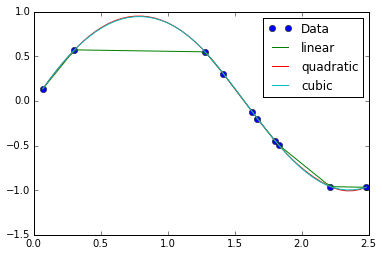
\includegraphics[height=7.5cm]{caso1.png}
    \caption{Interpolación lineal, cuadratica y cubica}
\end{figure}

\newpage

\paragraph{Caso 2}

Dados 20 puntos aleatorios entre $x=-10$ y $x=10$ para la función $f(x) = sin(x)/x$.

\begin{center}
\begin{boxedverbatim}

import numpy as np
import matplotlib.pyplot as plt
from scipy.interpolate import interp1d

# Original "data set" --- 20 random numbers between -10 and 10
# evaluated in sin(x)/x

x1 = np.random.random(20)
x2 = sorted(x1, key=float)
x3 = np.asarray(x2)
x0 = x3 * 20 - 10
y0 = sin(x0)/x0

plt.plot(x0, y0, 'o', label='Data')

# Array with points in between those of the data set
# for interpolation.

x = np.linspace(min(x0),max(x0),50)

# Available options for interp1d
options = ('linear', 'quadratic', 'cubic')

for o in options:
    f = interp1d(x0, y0, kind=o)  # interpolation function
    plt.plot(x, f(x), label=o)    # plot of interpolated data

plt.legend()
plt.show()
\end{boxedverbatim}
\end{center}

\begin{figure}[H]
    \centering
	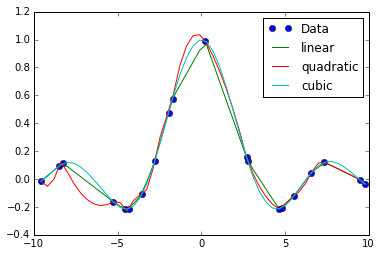
\includegraphics[height=7.5cm]{caso2.png}
    \caption{Interpolación lineal, cuadratica y cubica}
\end{figure}


\newpage

\paragraph{Caso 3}

Dados 16 puntos aleatorios entre $x=-3$ y $x=3$ para la función $f(x) = x^2 sin(2 x)$.

\begin{center}
\begin{boxedverbatim}

import numpy as np
import matplotlib.pyplot as plt
from scipy.interpolate import interp1d

# Original "data set" --- 16 random numbers between -3 and 3
# evaluated in x^2 sin(2 x)

x1 = np.random.random(16)
x2 = sorted(x1, key=float)
x3 = np.asarray(x2)
x0 = x3 * 6 - 3
y0 = x0**2 * sin(2*x0)

plt.plot(x0, y0, 'o', label='Data')

# Array with points in between those of the data set
# for interpolation.

x = np.linspace(min(x0),max(x0),50)

# Available options for interp1d
options = ('linear', 'quadratic', 'cubic')

for o in options:
    f = interp1d(x0, y0, kind=o)  # interpolation function
    plt.plot(x, f(x), label=o)    # plot of interpolated data

plt.legend()
plt.show()
\end{boxedverbatim}
\end{center}

\begin{figure}[H]
    \centering
	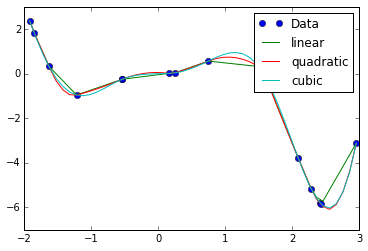
\includegraphics[height=7.5cm]{caso3.png}
    \caption{Interpolación lineal, cuadratica y cubica}
\end{figure}

\newpage

\paragraph{Caso 4}

Dados 12 puntos aleatorios entre $x=-2$ y $x=2$ para la función $f(x) = x^3 sin(3 x)$.


\begin{center}
\begin{boxedverbatim}

import numpy as np
import matplotlib.pyplot as plt
from scipy.interpolate import interp1d

# Original "data set" --- 12 random numbers between -2 and 2
# evaluated in x^3 sin(3x)

x1 = np.random.random(12)
x2 = sorted(x1, key=float)
x3 = np.asarray(x2)
x0 = x3 * 4 - 2
y0 = x0**3 * sin(3*x0)

plt.plot(x0, y0, 'o', label='Data')

# Array with points in between those of the data set
# for interpolation.

x = np.linspace(min(x0),max(x0),50)

# Available options for interp1d
options = ('linear', 'quadratic', 'cubic')

for o in options:
    f = interp1d(x0, y0, kind=o)  # interpolation function
    plt.plot(x, f(x), label=o)    # plot of interpolated data

plt.legend(loc='best')
plt.show()
\end{boxedverbatim}
\end{center}

\begin{figure}[H]
    \centering
	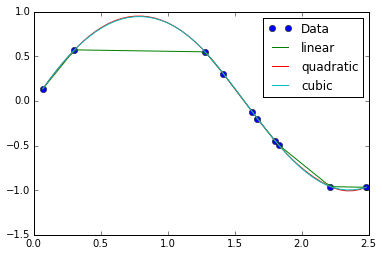
\includegraphics[height=7.5cm]{caso1.png}
    \caption{Interpolación lineal, cuadratica y cubica}
\end{figure}

\newpage

\section*{Conclusiones}

En esta actividad aprendimos a interpolar en Python usando con ayuda de la función \textbf{scipy.interpolate}, en especifico la clase \textbf{interp1d} que interpola una función 1-D. Deseamos obtener el valor de la variable dependiente en un punto donde no tenemos una muestra de la variable independiente. Interp1d toma dos argumentes, los valores x y y que seran usados para la interpolacion y lo que hace es que genera un objeto parecido a una funcion que nos da un estimado del valor de y, para los puntos definidos en que queremos el estimado. Notamos que las funciones interpoladas son continuas, siempre pasan por los puntos y que el ajuste empeora en las orillas. El siguiente paso sería encontrar la manera de que Python te de la función en sí.

\begin{thebibliography}{9}

\bibitem{pyman}
  SciPy,
  \emph{SciPy.Interpolate}, \\
  http://docs.scipy.org/doc/scipy/reference/tutorial/interpolate.html
  
\bibitem{sci}
  SciPy CookBook,
  \emph{Interpolation with Python}, \\
  http://scipy-cookbook.readthedocs.org/items/Interpolation.html
  
  \bibitem{pcn}
  PCN Upenn,
  \emph{Physical Modeling with Python}, \\
  physicalmodelingwithpython.blogspot.mx/2015/06/interpolation.html

\end{thebibliography}


\end{document}
